\deu{\section{Funktionen}\index{Funktionen}}
\eng{\section{Functions}\index{Functions}}
\setcounter{aufgabenNummer}{1}
\renewcommand{\kAufgabenBuchstabe}{F}


\subsection{\deu{Grundlagen}\eng{Basics}}

\kTrainingAufgabe{
\eng{translate:}
\textbf{Graphen Zeichenen}
Zeichnen Sie den Graphen der Funktion im Bereich $-4 \le{} x \le{} 4$.

a) $y=\frac12\cdot{}x$ \hspace{30mm}
b) $y=\frac1x$ \hspace{30mm}
c) $y=x^2$

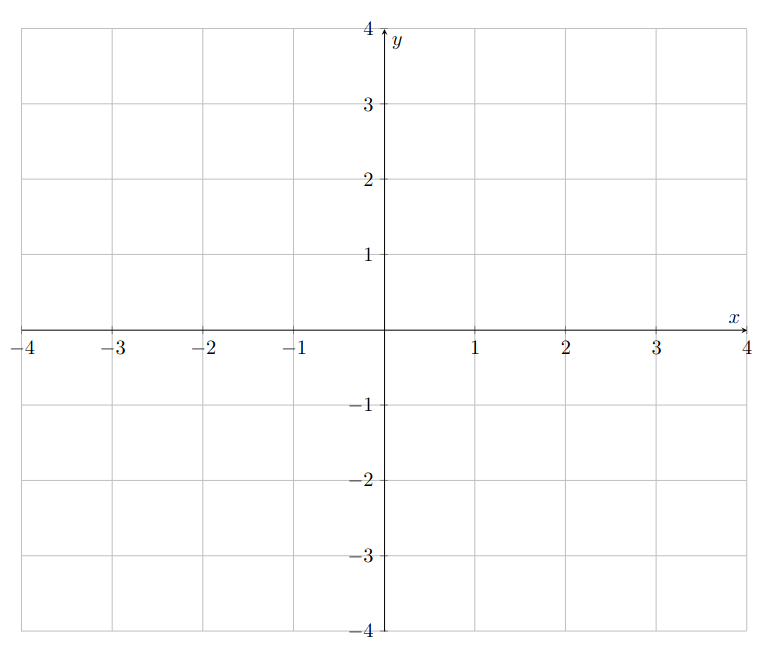
\includegraphics[width=150mm]{img/fct/Fct_ssA01.png}

}{%% Lösung
\raisebox{-80mm}{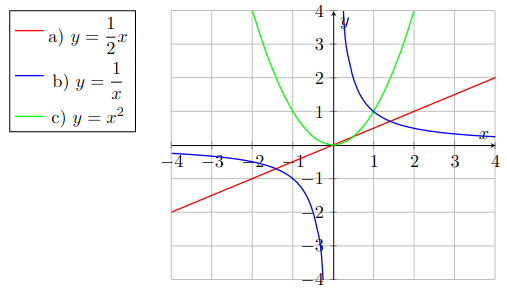
\includegraphics[width=150mm]{img/fct/Fct_ssL01.png}}
}{8}


\kTrainingAufgabe{
\eng{translate:}
\textbf{Funktionen auswerten}
Werten Sie den Funktionsterm $y=x^2-2x-5$ für folgende $x$-Werte aus:

a) $\frac12$ \hspace{25mm}
b) $-1$ \hspace{25mm}
c) $-\frac12$ \hspace{25mm}
d) $-\frac34$ \hspace{25mm}

}{%% Lösung
a) $-\frac{23}4$ \hspace{25mm}
b) $-2$ \hspace{25mm}
c) $-\frac{15}{4}$ \hspace{25mm}
d) $-\frac{47}{16}$ \hspace{25mm}
}{8}

\subsection{\deu{Lineare Funktionen}\eng{Linear Functions}}

\kTrainingAufgabe{
\eng{translate:}
\textbf{Steigungsbegriff, Mittelpunkt einer Strecke}

\kKommentar{Mittelpunkt ist ein geometrisches Konzept. Kommt das im
Rahmenlehrpln vor?}

a) Bestimmen Sie die Steigungen der Strecken a bis i. Zeichnen Sie
Steigungsdreiecke ein.

b) Bestimmen Sie die Koordinaten des Mittelpunkts jeder Strecke.

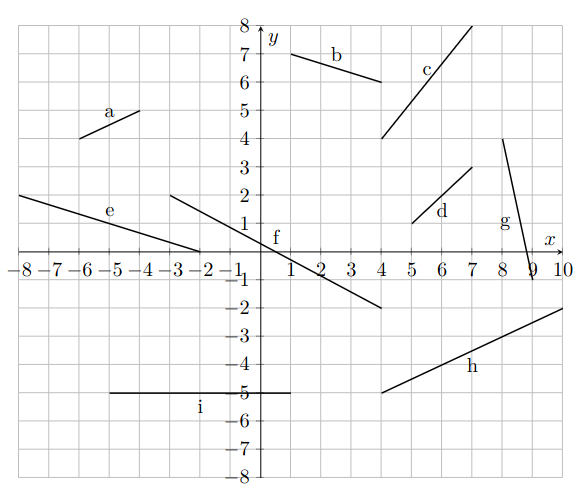
\includegraphics[width=130mm]{img/fct/Fct_ssA03.png}
}{%% Lösung

\renewcommand{\arraystretch}{2}
\begin{tabular}{|c|c|c|c|c|c|c|c|c|c|}\hline
   & a & b &c &d &e &f &g &h &i\\\hline
$a=m=$ & $\frac12$ & $\frac{-1}3$ & $\frac43$ & $1$ & $\frac{-1}3$
& $\frac{-4}7$ & $-5$ & $\frac12$ & $0$\\\hline
M.: & $(-5|\frac92)$ & $(\frac52|6.5)$ & $(5.5|6)$ & $(6|2)$ &
$(-5|1)$ & $(\frac12|0)$ & $(8.5|\frac32)$ & $(7|\frac{-7}2)$ & $(-2|-5)$\\\hline
 \end{tabular}
\renewcommand{\arraystretch}{2}
 
}{8}

\kTrainingAufgabe{
\eng{translate:}
\textbf{Graph zeichnen, Achsenschnittpunkte einzeichnen}:
Zeichnen Sie die Graphen folgen-
der Funktionen und heben Sie den Schnittpunkt mit der y-Achse und die Nullstelle hervor.
a) $y=2x+1$ \hspace{25mm}
b) $y=-x+3$ \hspace{25mm}
c) $y=-0.5x+4$ \hspace{25mm}

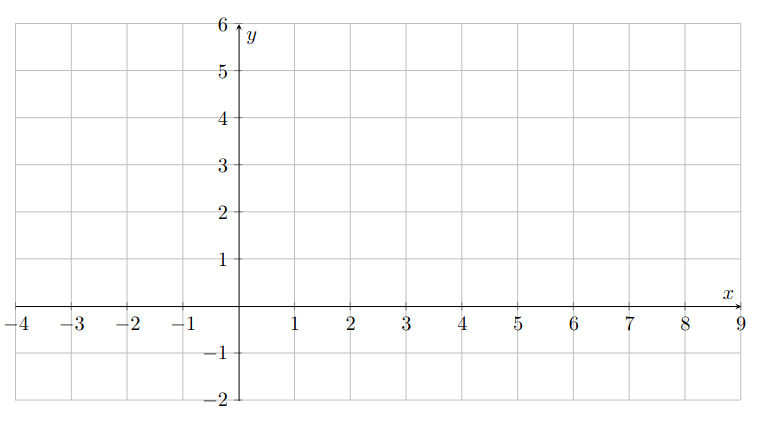
\includegraphics[width=150mm]{img/fct/Fct_ssA04.png}
}{%% Lösung

\raisebox{-50mm}{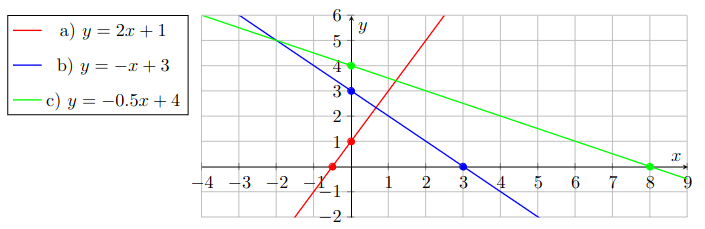
\includegraphics[width=150mm]{img/fct/Fct_ssL04.png}}

}{8}



\kTrainingAufgabe{
\eng{translate:}
\textbf{Funktionsterm auswerten:} Werten Sie die Funktion $f(x) = 2x+1$ für folgende Argumente
aus: $2$, $-2$, $0.5$, $-0.5$.
}{%% Lösung
$f(2)= 5$ \hspace{10mm}
$f(-2)=-3$ \hspace{10mm}
$f(0.5) = 2$ \hspace{10mm}
$f(-0.5)=0$
}{8}





\kTrainingAufgabe{
\eng{translate:}
\textbf{Bedeutung der Parameter; explizite Form:} Bestimmen Sie Steigung und $y$-
Achsenabschnitt in der durch die Funktionsgleichung $3x-2y=60$ gegebenen Geraden.

}{%% Lösung
$$y = 1.5x - 30$$
Steigung = 1.5 und $y$-Achsenabschnitt = -30.
}{8}





\kNiveauAufgabe{
\eng{translate:}\textbf{Achsenschnittpunkte berechnen:}
Berechnen Sie die Achsenschnittpunkte der Geraden $g$
mit der Funktionsgleichung $y=-0.25x+4$.
}{%% Lösung
Mit $x$-Achse: $(0|4)$

Mit $y$-Achse: $(16|0)$
}{8}





\kTrainingAufgabe{
\eng{translate:}\textbf{Horizontale Gerade:}
Notieren Sie die Funktionsgleichung der horizontalen Geraden durch den Punkt $P=(5|8)$.
}{%% Lösung
$f(x) = y = 8$
}{8}





\kNiveauAufgabe{
\eng{translate:}\textbf{Zweipunkteaufgabe:}
Wie lautet die Funktionsgleichung der Geraden, die durch folgende
zwei Punkte läuft (Resultate exakt angeben)?

a) $A(5|8)$ und $B(7|12)$


b) $A(-3|4)$ und $B(2|1)$


c) $A(-1|1)$ und $B(10|5)$

}{%% Lösung
a) $A=(5|8)$ und $B=(7|12)$ $\Longrightarrow$  $y=2x-2$


b) $A=(-3|4)$ und $B=(2|1)$ $\Longrightarrow$ $y=\frac{-3}5x+\frac{11}5$


c) $A=(-1|1)$ und $B=(10|5)$ $\Longrightarrow$  $y=\frac4{11}x+\frac{15}{11}$
}{8}




\kTrainingAufgabe{
\eng{translate:}\textbf{Funktionsgleichung aus Grafik bestimmen}
Wie lauten die Funktionsgleichungen der Geraden $a$ bis $f$?

\kKommentar{Niveau Aufnahmeprüfung!}

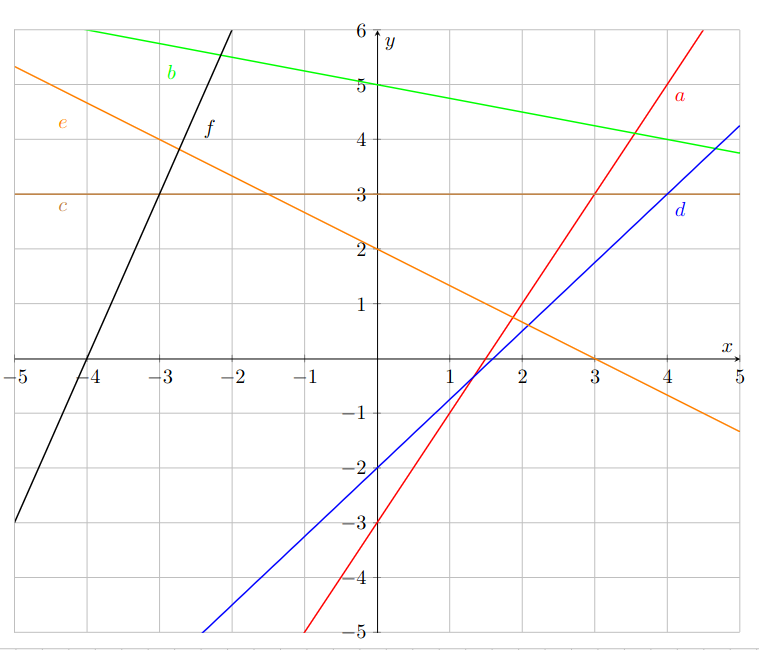
\includegraphics[width=140mm]{img/fct/Fct_ssA10.png}

}{%% Lösung
\raisebox{-80mm}{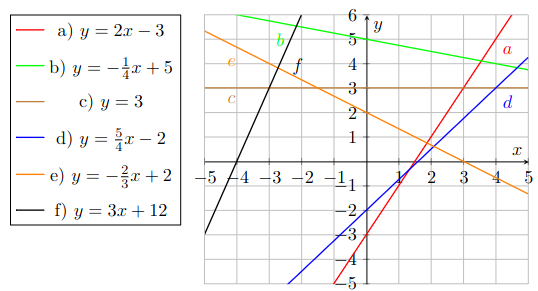
\includegraphics[width=160mm]{img/fct/Fct_ssL10.png}}
}{8}





\kNiveauAufgabe{
\eng{translate:}\textbf{Achsenschnittpunkte berechnen}
Berechnen Sie die Schnittpunkte des Graphen mit den beiden
Koordinatenachsen.

a) $y=10-3x$ \hspace{30mm}
b) $y=5-\frac12x$ \hspace{30mm}
c) $y=\frac{10x-2}5$ 
}{%% Lösung

\renewcommand{\arraystretch}{2}
\begin{tabular}{c|c|c|c}
& a) $y=10-3x$ & b) $y=5-\frac12x$ & c) $y=\frac{10x-2}5$  \\\hline
$N(x_n|0)$ & $\left(\frac{10}3\middle|0\right)$ & $(10|0)$ &
$(\frac15|0)$ \\\hline
$B(0|b)$ & $(0|10)$ & $(0|5)$ & $\left(0\middle|\frac{-5}2\right)$
 \end{tabular}
 
\renewcommand{\arraystretch}{2}

}{8}






\kTrainingAufgabe{
\eng{translate:}\textbf{Umwandeln in die explizite Form}
Wandeln Sie die Funktionsgleichung in die explizite Form $y=ax+b$
(bzw. $y=mx+q$) um.

a) $y=2-\frac{x}2$

b) $y=\frac{2x-10}3$

c) $y=\frac{1-x}{12}$

d) $y = -(2+1.25x)$

e) $4y-3x = 1.5$
}{%% Lösung

a) $y=\frac{-1}2\cdot{}x + 2$

b) $y=\frac23\cdot{}x - \frac{10}3$

c) $y=\frac{-1}{12}\cdot{}x + \frac1{12}$

d) $y=\frac{-5}4\cdot{}x - 2$

e) $y=\frac34\cdot{}x + \frac38$
}{8}





\kNiveauAufgabe{
\eng{translate:}\textbf{Liegt $P (-4.5|7)$ auf, oberhalb oder unterhalb der Geraden $g$?}

a) $g: y=-2x-2$

b) $g: y= -0.5x + 4.7$

c) $g: y = 2.5x + 18.25$
}{%% Lösung

a) Punkt liegt \textbf{auf} der Geraden.  

b) Punkt liegt \textbf{oberhalb} der Geraden.  

c) Punkt liegt \textbf{auf} der Geraden.  

}{8}




\kNiveauAufgabe{
\eng{translate:}\textbf{Geradengleichung aus Steigung und einem Punkt
$P \in g$ (Punkt-Steigungs-Aufgabe)}

Eine Gerade $g$ hat die Steigung $-0.4$ und geht durch $P (-2| -7)$. Wie lautet
die Funktionsgleichung von $g$?
}{%% Lösung
$g : y = -0.4x - 7.8$
}{8}




\kNiveauAufgabe{
\eng{translate:}\textbf{Liegen drei gegebene Punkte auf einer gemeinsamen Geraden oder nicht?}
Liegen $A(-2.5| -20.8)$, $B(21.5|50.0)$ und $C(100.0|281.575)$ auf
einer gemeinsamen Geraden $g$ oder nicht? Begründung?
}{%% Lösung
Ja, die Steigung von $AB$ ist gleich der Steigung von $BC$, nämlich $2.95$.
}{8}




\kNiveauAufgabe{
\eng{translate:}\textbf{Fehlende Punktkoordinate bestimmen: }
Der Punkt $C(-12.5|y_C)$ liegt auf der Geraden
$g$ durch $A(-2.5| - 20.8)$ und $B(21.5|50.0)$. Wie lautet die Koordinate $y_C$?
}{%% Lösung

$y_C = -50.3$
}{8}




\kNiveauAufgabe{
\eng{translate:}\textbf{Geradengleichung einer zur gegebenen Geraden parallelen Geraden durch einen
Punkt bestimmen:}
Gegeben ist $g : y = 4.8x - 2$. Die Gerade $h$ ist parallel zu $g$ und läuft
durch den Punkt $P(-8|2)$. Wie lautet die Geradengleichung von $h$?
}{%% Lösung
$h : y = 4.8x + 40.4$
}{8}




\kNiveauAufgabe{
\eng{translate:}\textbf{Schnittpunkt S zweier Geraden berechnen:}

Berechnen Sie den Schnittpunkt von $g: \frac{-2}3x+5$ und $h: \frac{-3}4x+10$
}{%% Lösung
Schnittpunkt = $(180|125)$
}{8}



\textbf{Kombinationen obiger Grundaufgaben}

\kNiveauAufgabe{
\eng{translate:}Die Gerade g hat die Steigung $-0.5$ und die Nullstelle bei $x = 5$. Wie lautet die Funktions-
gleichung von $g$?

}{%% Lösung
$g : y = -0.5x + 2.5$
}{8}




\kNiveauAufgabe{
\eng{translate:}Die Gerade $g$ hat die Steigung $-3$. Ferner liegt $A(-2|4)$ auf $g$. Der Punkt $B(x_B | - 23)$ liegt
ebenfalls auf $g$. Wie lautet die Koordinate $x_B$?

}{%% Lösung
$x_B = 7$
}{8}




\kNiveauAufgabe{
\eng{translate:}Die Gerade $g$ geht durch $A(1|5)$ und $B(8| - 2)$. Die Gerade $h$ schneidet die $x$-Achse im
selben Punkt $N$ wie die Gerade $g$. Die Gerade $h$ hat ferner die Steigung $4$. Wie lautet die
Funktionsgleichung von $h$?

}{%% Lösung
$h : y = 4x - 24$
}{8}


\textbf{Angewandte lineare Funktionen}

\kNiveauAufgabe{
\eng{translate:}Eine Taxifahrt von 10 km kostet CHF 21, eine solche von 15 km aber CHF 27. Wie lautet
die lineaer Funktionsgleichung $y = f (x)$ mit $x$ = Anzahl km Fahrstrecke und $y$ = Anzahl CHF
Gesamttaxe? Variante: Gesucht die Funktionsgleichung $K = f (s)$, $K$ = Kosten in CHF, $s$ =
Strecke in km. Es werden beide Varianten akzeptiert.

}{%% Lösung

$y = 1.2x + 9 $

oder (Variante)

$K(s) = 1.2 \text{CHF/km} · s + 9 \text{CHF}$

}{8}





\kNiveauAufgabe{
\newcommand{\tempGrad}[1]{${}^{\circ{}}$#1}
\eng{translate:}Die englische Temperaturskala (Fahrenheit-Grade, \tempGrad{F}) ist wie folgt festgelegt:
0\tempGrad{C} (Celsius) entsprechen 32 \tempGrad{F} (Fahrenheit). 100 \tempGrad{C}
entsprechen 212 \tempGrad{F}.

a) Wie lautet die lineare Funktionsgleichung zur Umrechnung
von \tempGrad{C} (= $x$) in \tempGrad{F} (= $y$)?

b) Wie lautet die lineare umgekehrte Funktion zur Umrechnung von \tempGrad{F}(= $x$) in \tempGrad{C} (= $y$)?

}{%% Lösung
a) $y = 1.8x + 32$

b) $y= \frac95 x - \frac{160}9$
}{8}





\kNiveauAufgabe{
\eng{translate:}
Eine lineare Notenskala ist wie folgt festgelegt:
Für 24 Punkte gibt es Note 6, für 0 Punkte Note 1.

a) Wie lautet die lineare Notenfunktion $y = f (x)$? $x$ = Anzahl Punkte, $y$ = Notenzahl.

b) Welche Note (auf 1 Dezimale gerundet) wird mit 18 Punkten erreicht?

c) Wie viele Punkte ergeben die Note 4?
}{%% Lösung

a) $y=\frac5{24}x+1$

b) $4.8$

c) 14.4 Punkte
}{8}





\kNiveauAufgabe{
\eng{translate:}\textbf{}
Lineare Abschreibung einer Maschine: Eine Maschine mit Neuwert CHF 5’000.- wird linear
abgeschrieben: Jedes Jahr soll sich ihr Wert um CHF 250.- verringern.

a) Wie lautet die lineare Abschreibungsfunktion $y = f (x)$ mit $x$ = Anzahl Jahre und $y$ =
Anzahl CHF Zeitwert nach $x$ Jahren?

b) Nach wie vielen Jahren ist die Maschine vollständig abgeschrieben?
}{%% Lösung

a) $y = -250x + 5000$

b) Nach 20 Jahren.
}{8}





\kNiveauAufgabe{
\eng{translate:}\textbf{}
Für HD-TV via Internet wird neben einer Grundgebühr auch die Anzahl Stunden, während
derer man fernsieht, verrechnet. Anbieter A verlangt pro Monat eine Grundgebühr von CHF
5.- und pro Stunde fernsehen eine Gebühr von 20 Rappen. Anbieter B verlangt folgendes:
Bei 20 h fernsehen CHF 10.- und bei 100 h fernsehen CHF 20.- (beides inkl. Grundgebühr).
Wie lauten die beiden Kostenfunktionen? $x$ = Anzahl Stunden Fernsehzeit, $y$ = Anzahl CHF
Kosten. Bei welcher Stundenzahl sind beide Anbieter gleich teuer?
}{%% Lösung
Gleicher Preis bei 33 Stunden und 20 Minuten.
}{8}



\subsubsection{Grafisches Lösen von Gleichungssystemen}


\kNiveauAufgabe{
\eng{translate:}
Lösen Sie das Gleichungssystem grafisch und interpretieren Sie die
Lösung:

a) \gleichungZZ{3x-4y}{8}{y}{\frac14 x + 6}

\begin{center}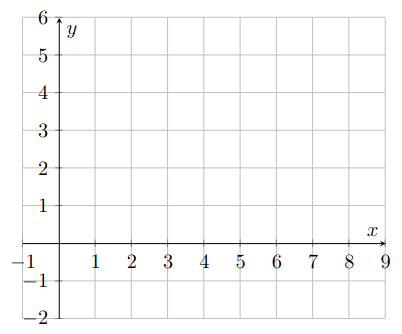
\includegraphics[width = 100mm]{img/fct/Fct_ssA27a.png}\end{center}


b) \gleichungZZ{10y}{7.5x}{18.75x+25y}{1500}

\begin{center}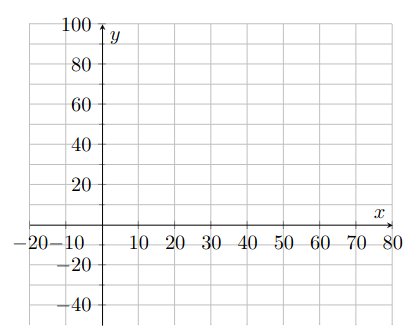
\includegraphics[width = 100mm]{img/fct/Fct_ssA27b.png}\end{center}

c) \gleichungZZ{13x+y-9.5}{4y-\frac{28}7}{-\frac45y+x}{-5+0.2x}

\begin{center}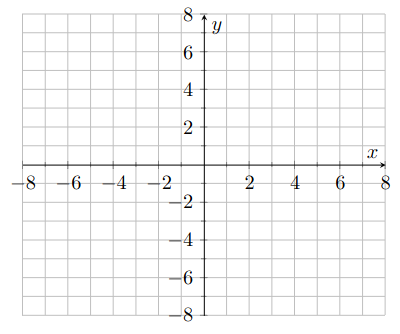
\includegraphics[width = 100mm]{img/fct/Fct_ssA27c.png}\end{center}

d) \gleichungZZ{40}{-2y-x}{3.5x-5y+82}{4\left(x-y+\frac{51}2\right)}

\begin{center}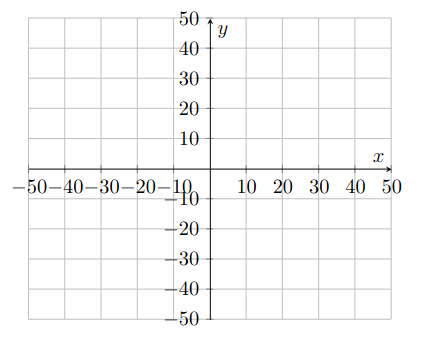
\includegraphics[width = 100mm]{img/fct/Fct_ssA27d.png}\end{center}

}{%% Lösung

a) \gleichungZZ{3x-4y}{8}{y}{\frac14 x + 6} $$S=(8|4)$$

\begin{center}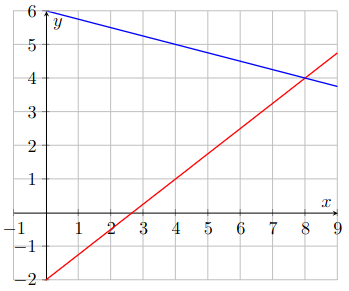
\includegraphics[width = 100mm]{img/fct/Fct_ssL27a.png}\end{center}


b) \gleichungZZ{10y}{7.5x}{18.75x+25y}{1500} $$S=(40|30)$$

\begin{center}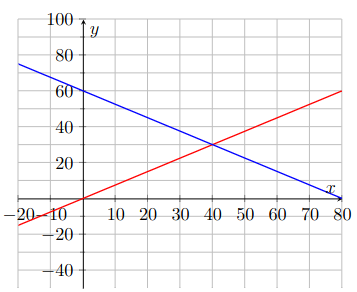
\includegraphics[width = 100mm]{img/fct/Fct_ssL27b.png}\end{center}

c) \gleichungZZ{13x+y-9.5}{4y-\frac{28}7}{-\frac45y+x}{-5+0.2x}

$$\mathbb{L}_S = \left\{\right\}$$

\begin{center}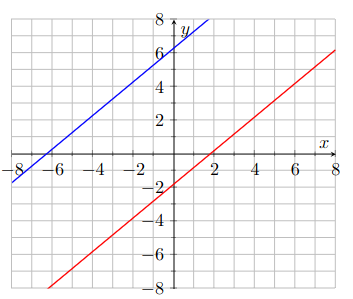
\includegraphics[width = 100mm]{img/fct/Fct_ssL27c.png}\end{center}

d) \gleichungZZ{40}{-2y-x}{3.5x-5y+82}{4\left(x-y+\frac{51}2\right)}

Die Geraden sind zusammenfallend. 

\begin{center}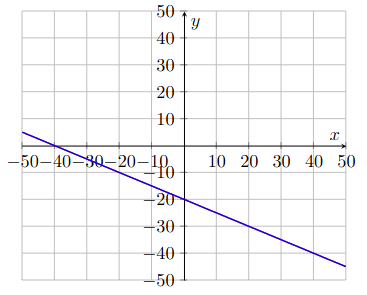
\includegraphics[width = 100mm]{img/fct/Fct_ssL27d.png}\end{center}

}{2}
\newpage






\subsection{\deu{Potenzfunktionen}\eng{Power Functions}}
\kKommentar{Graphen von Potenzfunktionen sind Hyperbeln oder
  Parabeln...}
  
\kKommentar{...Dies in den Titeln korrekt vermerken (nicht
  Hyperbelfunktion etc.)}

\subsubsection{$n>1$: \deu{Parabeln}\eng{Parabolas}}

\kNiveauAufgabe{
\deu{Zeichnen Sie den Graphen folgender Potenzfunktionen:}
\eng{Draw the graph of the following power functions:}
a) $x \mapsto 0.5x^3$  \hspace{30mm}  b) $x\mapsto -x^4$

\begin{tabular}{cc}
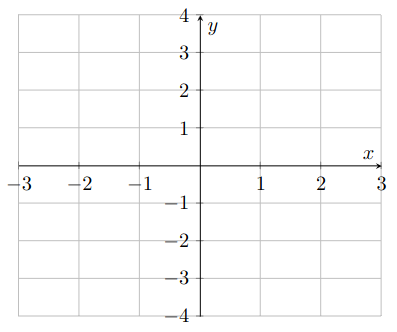
\includegraphics[width=85mm]{img/fct/Fct_ssA28a.png}
&
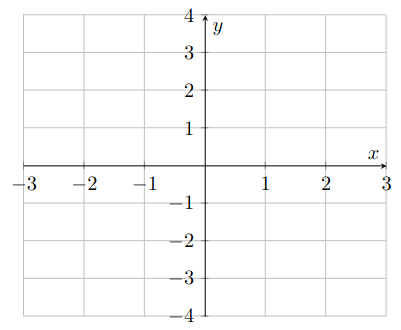
\includegraphics[width=85mm]{img/fct/Fct_ssA28b.png}
\\
 \end{tabular}
 

}{%% Lösung

\begin{tabular}{cc}
a)

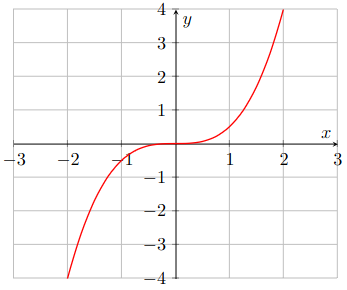
\includegraphics[width=70mm]{img/fct/Fct_ssL28a.png}
&b)

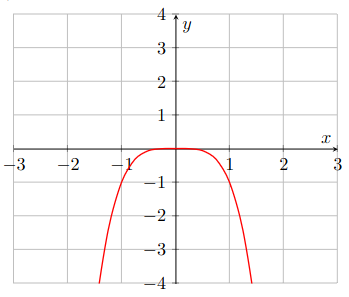
\includegraphics[width=70mm]{img/fct/Fct_ssL28b.png}
\\
 \end{tabular}

}{4}


\kNiveauAufgabe{
\deu{Bestimmen Sie den Faktor $a$ in 
$x\mapsto a\cdot{}x^4$ wenn der Graph durch den Punkt $A(3|3)$ verläuft.}
\eng{Determine the factor $a$ in $x\mapsto a \cdot x^4$ when the graph
passes through the point $A(3|3)$.}
}{%% Lösung
$3=3\cdot{}a^4 \Longrightarrow a=\frac1{27}$
}{6}%% end KNiveauAufgabe



\subsection{Exponentialfunktionen}

\subsubsection{Wachstum und Zerfall}

\subsubsection{Sättigung}
\newpage
